\documentclass[conference]{IEEEtran}
\IEEEoverridecommandlockouts

\usepackage{fontspec}
\setmainfont{texgyretermes}[Extension=.otf,UprightFont=*-regular,BoldFont=*-bold,ItalicFont=*-italic,BoldItalicFont=*-bolditalic]
\setmonofont[Scale=0.92]{Inconsolatazi4-Regular.otf}[BoldFont=Inconsolatazi4-Bold.otf]
\usepackage{cite}
\usepackage{amsmath,amssymb}
\usepackage{unicode-math}
\setmathfont{texgyretermes-math.otf}
\usepackage{graphicx}
\graphicspath{{../ui/shots/}}
\usepackage{booktabs}
\usepackage{array}
\usepackage{multirow}
\usepackage{textcomp}
\usepackage{xcolor}
\usepackage{listings}
\usepackage{tikz}
\usetikzlibrary{positioning,arrows.meta,fit,backgrounds}
\usepackage{url}
\usepackage[hidelinks]{hyperref}

\definecolor{kw}{RGB}{90,40,150}
\definecolor{cmt}{RGB}{110,110,110}
\definecolor{str}{RGB}{150,80,0}

\lstdefinelanguage{HomeLang}{
  morekeywords={IF,THEN,ELSE,END,WHEN,AT,ON,FOR,RULE,PRIORITY,ROOM,DEVICE,SENSOR,IN,UNIT,
    TURN_ON,TURN_OFF,TOGGLE,SET,TO,LOCK,UNLOCK,OPEN,CLOSE,WAIT,NOTIFY,AND,OR,NOT,IS,BETWEEN,
    SIMULATE,FROM,STEP,DETECTED,CHANGES,TURNS,RISES,FALLS,ABOVE,BELOW,WEEKDAYS,CLEAR,AWAY,HOME},
  sensitive=true,
  morecomment=[l]{//},
  morecomment=[s]{/*}{*/},
  morestring=[b]",
}
\lstset{
  basicstyle=\ttfamily\scriptsize,
  keywordstyle=\color{kw}\bfseries,
  commentstyle=\color{cmt}\itshape,
  stringstyle=\color{str},
  columns=fullflexible,
  keepspaces=true,
  breaklines=true,
  frame=single,
  framesep=2pt,
  xleftmargin=3pt,
  xrightmargin=3pt,
  aboveskip=4pt,
  belowskip=4pt,
  literate={°}{{\textdegree}}1,
}

\newcommand{\code}[1]{\texttt{#1}}
\newcommand{\degC}{\textdegree{}C}
\newcommand{\degF}{\textdegree{}F}

\begin{document}

\title{HomeLang: A Phase-by-Phase Visualized Compiler for a Smart-Home Trigger--Action Language}

% Force a new row of author blocks, each row centred on the page.
\makeatletter
\newcommand{\linebreakand}{%
  \end{@IEEEauthorhalign}\hfill\mbox{}\par
  \mbox{}\hfill\begin{@IEEEauthorhalign}}
\makeatother

\author{
\IEEEauthorblockN{Deepanshu Mehta}
\IEEEauthorblockA{\textit{Roll No. 230124} \\
Lexer, project scaffold, UI shell}
\and
\IEEEauthorblockN{Vishesh Rao}
\IEEEauthorblockA{\textit{Roll No. 230129} \\
Parser and grammar}
\and
\IEEEauthorblockN{Manu Vahan}
\IEEEauthorblockA{\textit{Roll No. 230125} \\
Semantic analysis}
\linebreakand
\IEEEauthorblockN{Pranay Vishwakarma}
\IEEEauthorblockA{\textit{Roll No. 230083} \\
Intermediate code and optimizer}
\and
\IEEEauthorblockN{Ankush Yadav}
\IEEEauthorblockA{\textit{Roll No. 230146} \\
Code generation, VM and simulator}
\linebreakand
\IEEEauthorblockA{\textit{B.Tech CSAI, Rishihood University} \\
Compiler Design Course Project \quad$\cdot$\quad Team \textit{Ghar} \\
\url{https://github.com/Deepanshu-Mehta/HomeLang-CompilerDesign}}
}

\maketitle

\begin{abstract}
We present HomeLang, a complete compiler for a domain-specific trigger--action language that automates a smart home, together with an interactive web application that exposes the output of every compilation phase. A program such as \code{IF TEMPERATURE > 30 THEN TURN\_ON AC} passes through seven stages: a maximal-munch lexer driven by six deterministic finite automata stored as data; a hand-written LL(1) recursive-descent parser whose grammar is machine-checked for conflicts; a semantic analyzer with a symbol table, a dimensional type system, interval analysis over disjunctive normal form, and loop detection with Tarjan's strongly connected components; quadruple three-address code produced with backpatching; nine optimization passes, each with a stated safety argument; bytecode generation for a stack virtual machine; and a discrete-event simulation that animates a floor plan. The compiler defines 74 diagnostic codes across lexical, syntactic, semantic and run-time errors, each with a position and a hint. Correctness is established by 1104 unit and golden tests, 56 browser tests, and a three-way differential test in which an AST interpreter, the unoptimized VM and the optimized VM must produce identical event logs on every example, 39 targeted programs and 400 random programs. On the optimizer demonstration program the passes reduce 60 quadruples to 31 and 16 jumps to 4. A full compilation of the largest example takes under 4\,ms.
\end{abstract}

\begin{IEEEkeywords}
compiler design, domain-specific language, LL(1) parsing, backpatching, interval analysis, code optimization, stack virtual machine, trigger--action programming, smart home, program visualization
\end{IEEEkeywords}

%=====================================================================
\section{Introduction}
%=====================================================================

Smart-home platforms let end users write rules of the form ``if something happens, then do something''. Ur et~al.\ found that 62.6\% of 1,590 smart-home behaviours requested by 318 participants were programming behaviours, and that all of them could be expressed as trigger--action rules provided that multiple triggers and actions were allowed~\cite{ur2014}. The same simplicity hides real bugs: Brackenbury et~al.\ catalogued ten classes of trigger--action bugs, including infinite loops, contradictory actions and missing reversals, and found that eight of them impaired users' ability to predict what their rules would do~\cite{brackenbury2019}.

This makes the domain a good fit for a compiler-design project. The language is small enough to specify completely, yet it needs every classical phase: tokens with units and times, a grammar with nested conditionals, a type system with physical dimensions, static detection of real bug classes, control-flow lowering, optimization, code generation, and a run-time model with precise timing rules.

HomeLang is built on the \emph{AI Product Engineering Track} of the course: the compiler is a single TypeScript application with an interactive interface in which a user types a program and sees, as they type, the output of every phase. The contributions of the project are:
\begin{enumerate}
  \item A fully specified trigger--action language with edge-triggered semantics, declarations, units, time windows, priorities, delays and a scenario block (Section~\ref{sec:lang}).
  \item A seven-stage compiler in which every phase is a pure function with a common result contract, and in which the lexer's automata and the parser's grammar are \emph{data} that both the compiler and the visualizer use (Sections~\ref{sec:arch}--\ref{sec:phases}).
  \item Static analyses that target documented trigger--action bug classes: contradictions, tautologies, rule conflicts with concrete witnesses, and cascade loops (Section~\ref{sec:sem}).
  \item A verification strategy, centred on three-way differential testing, that shows the optimizer preserves behaviour (Section~\ref{sec:testing}).
  \item An interactive, phase-by-phase walkthrough that shows tokens, DFA traces, parse trees, the AST, the symbol table, IR with backpatching, per-pass optimizer diffs, bytecode and a simulated home (Section~\ref{sec:ui}).
\end{enumerate}

%=====================================================================
\section{Background and Related Work}
%=====================================================================

\subsection{Trigger--action platforms}
Home Assistant structures an automation as triggers, conditions and actions; its numeric-state trigger fires when a value \emph{crosses} a threshold, not while it stays above it~\cite{homeassistant}. SmartThings and openHAB expose the same parts, and SmartThings adds \code{else} branches and delays; IFTTT reduces a rule to a trigger, optional filter code and actions. HomeLang adopts edge-triggered \code{IF} rules for the same reason these platforms do: a level-triggered rule re-fires on every sensor update, which Brackenbury et~al.\ call the \emph{repeated triggering} bug~\cite{brackenbury2019}. Device ranges in HomeLang's catalogue are informed by the Matter specification~\cite{matter}; for example, Matter's absolute cooling setpoint limits default to 16--32\,\degC, and HomeLang uses the course brief's narrower 16--30\,\degC{} for the AC.

\subsection{Verification of home automations}
IotSan translates SmartThings apps into Promela and model-checks them with Spin~\cite{iotsan}; AutoTap synthesises rule repairs from LTL properties~\cite{autotap}. These tools are far heavier than a course compiler. HomeLang instead implements lightweight static versions of the most important checks inside the semantic phase, with exact results for the single-variable conditions the language allows.

\subsection{Parser construction}
Parser generators such as ANTLR, Peggy, Chevrotain and Nearley were considered and rejected. They hide the automata, FIRST/FOLLOW sets and parse table, which are exactly what the walkthrough must show. Following the recursive-descent approach of production compilers and of \emph{Crafting Interpreters}~\cite{nystrom}, we hand-wrote an LL(1) parser in which each grammar rule is one function. Intermediate code and backpatching follow Aho et~al.~\cite{dragon}, and loop detection uses Tarjan's algorithm~\cite{tarjan}.

%=====================================================================
\section{The HomeLang Language}\label{sec:lang}
%=====================================================================

\subsection{Programs}
A program has optional declarations, then rules, then an optional \code{SIMULATE} block. With no declarations, a \emph{standard home} is loaded (four rooms; devices \code{AC}, \code{LIGHT}, \code{FAN}, \code{DOOR}, \code{CURTAIN}; sensors \code{TEMPERATURE}, \code{HUMIDITY}, \code{MOTION}, \code{CONTACT}, \code{PRESENCE}), so the one-line brief compiles on its own. Any declaration switches the prelude off and only declared names exist. Listing~\ref{lst:adv} shows the three rule kinds: state rules (\code{IF}), event rules (\code{WHEN}) and time rules (\code{AT}).

\begin{lstlisting}[language=HomeLang,caption={Extract of \code{examples/advanced.home}.},label={lst:adv}]
ROOM BEDROOM; ROOM ENTRANCE;
DEVICE AC : AIR_CONDITIONER IN BEDROOM;
SENSOR TEMP : TEMP_SENSOR IN BEDROOM UNIT C;
SENSOR MOTION : MOTION_SENSOR IN BEDROOM;

RULE "Cool bedroom" PRIORITY 2:
IF TEMP > 86F AND (MOTION IS DETECTED
   OR TIME BETWEEN 22:00 AND 06:00) FOR 2MIN THEN
  TURN_ON AC, SET AC TEMPERATURE TO 24C
ELSE TURN_OFF AC END;

RULE "Morning":
AT 07:00 ON WEEKDAYS THEN OPEN CURTAIN END;

SIMULATE FROM 21:30 TO 07:30 STEP 1MIN {
  AT 21:30: TEMP = 29C, MOTION = CLEAR;
  AT 22:15: TEMP = 31C;
}
\end{lstlisting}

\subsection{Types and units}
HomeLang has five types. A \emph{quantity} is a number with a dimension: temperature, percent, illuminance, duration, colour temperature or a unitless count. Comparison and addition are defined only within one dimension, and multiplication and division only by a count. \emph{Time} is minutes 0--1439, and \code{BETWEEN} on times is a half-open window $[a, b)$ that wraps midnight. \emph{Day} is \code{MON}--\code{SUN}. \emph{Enum} is the state set of a device or sensor and has no ordering. \emph{Boolean} appears only as a whole condition. Temperatures are stored in \degC{} and durations in seconds, so \code{86F} is converted at compile time. A bare number takes the unit of the value it meets, and note W415 records this.

\subsection{Run-time semantics}
An \code{IF} rule runs its \code{THEN} branch when its condition changes from false to true and its \code{ELSE} branch when it changes back. \code{FOR} requires the condition to hold for the whole duration; if it drops first, the hold is cancelled. Within one round, triggered rules run in source order against the current values, and their commands are queued and then resolved per device: the highest \code{PRIORITY} wins, then the later rule in source order. Every committed device change is an event for the next round, up to a cascade depth of 16, beyond which run-time error R501 stops the simulation. A rule in \code{WAIT} ignores new triggers, like Home Assistant's \code{single} mode; a state rule is re-evaluated once when it finishes, so an edge missed while it was busy is not lost.

%=====================================================================
\section{System Architecture and Methodology}\label{sec:arch}
%=====================================================================

\begin{figure*}[t]
\centering
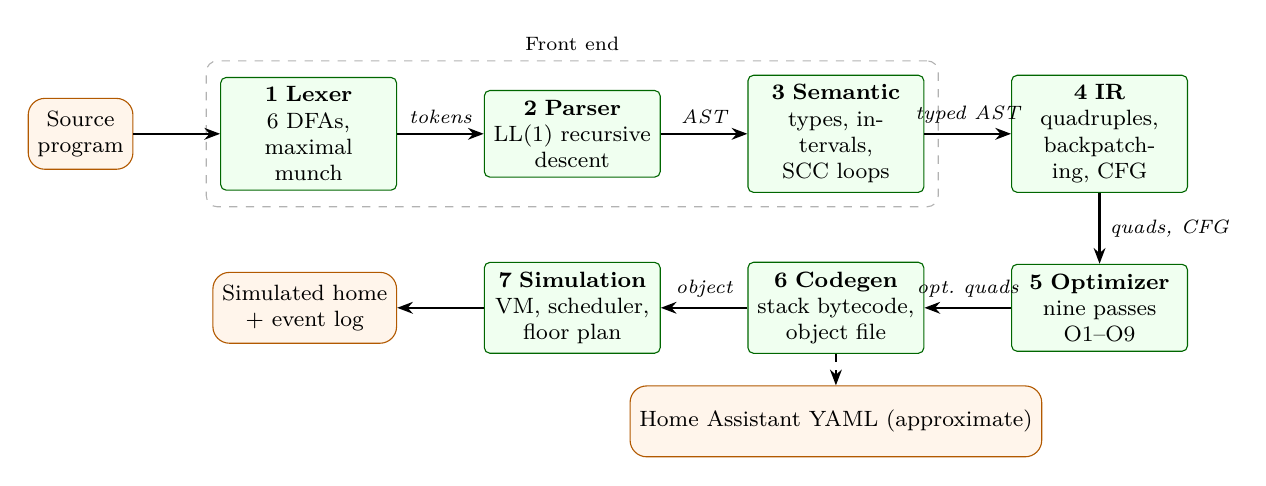
\begin{tikzpicture}[
  node distance=4mm and 11mm,
  st/.style={draw=green!40!black, fill=green!6, rounded corners=2pt, align=center, font=\footnotesize, minimum height=11mm, text width=20mm},
  ep/.style={draw=orange!70!black, fill=orange!8, rounded corners=6pt, align=center, font=\footnotesize, minimum height=9mm},
  lab/.style={font=\scriptsize\itshape, midway, above},
  ar/.style={-{Stealth[length=2mm]}, thick}
]
\node[ep] (src) {Source\\program};
\node[st, right=of src] (lex) {\textbf{1 Lexer}\\6 DFAs,\\maximal munch};
\node[st, right=of lex] (par) {\textbf{2 Parser}\\LL(1) recursive\\descent};
\node[st, right=of par] (sem) {\textbf{3 Semantic}\\types, intervals,\\SCC loops};
\node[st, right=of sem] (ir) {\textbf{4 IR}\\quadruples,\\backpatching, CFG};
\node[st, below=9mm of ir] (opt) {\textbf{5 Optimizer}\\nine passes\\O1--O9};
\node[st, left=of opt] (gen) {\textbf{6 Codegen}\\stack bytecode,\\object file};
\node[st, left=of gen] (sim) {\textbf{7 Simulation}\\VM, scheduler,\\floor plan};
\node[ep, left=of sim] (home) {Simulated home\\+ event log};
\node[ep, below=4mm of gen] (ha) {Home Assistant YAML (approximate)};
\draw[ar] (src) -- (lex);
\draw[ar] (lex) -- node[lab]{tokens} (par);
\draw[ar] (par) -- node[lab]{AST} (sem);
\draw[ar] (sem) -- node[lab]{typed AST} (ir);
\draw[ar] (ir) -- node[right, font=\scriptsize\itshape]{quads, CFG} (opt);
\draw[ar] (opt) -- node[above, font=\scriptsize\itshape]{opt.\ quads} (gen);
\draw[ar] (gen) -- node[above, font=\scriptsize\itshape]{object} (sim);
\draw[ar] (sim) -- (home);
\draw[ar, dashed] (gen) -- (ha);
\begin{scope}[on background layer]
\node[draw=gray!60, dashed, rounded corners, fit=(lex)(par)(sem), inner sep=5pt, label={[font=\scriptsize]above:Front end}] {};
\end{scope}
\end{tikzpicture}
\caption{The HomeLang pipeline. Every stage returns \code{\{status, output, diagnostics, timeMs\}}. A stage with errors stops the pipeline and later stages are reported as skipped; warnings do not stop it.}
\label{fig:pipeline}
\end{figure*}

\subsection{A pure compiler core}
The compiler (\code{src/compiler/}) is a set of pure functions with no knowledge of the page. One public module, \code{index.ts}, exports \code{compile(source)}, which returns the seven stage results of Fig.~\ref{fig:pipeline}, and \code{createSession()} for the live simulation. The web interface, the command-line tool and the tests all go through this module, and a test fails if the UI imports anything else. Every phase therefore has a single, testable contract, and the command line can emit any intermediate state:
\begin{lstlisting}[language=bash]
npm run homelang -- compile examples/brief.home \
    --emit=tokens|ast|symbols|ir|opt|bytecode|sim
\end{lstlisting}

\subsection{Shared data instead of duplicated logic}
The six lexer automata, the grammar, and the device catalogue are plain data objects. The lexer executes the automata; the UI draws the same objects as state diagrams. The LL(1) checker computes FIRST and FOLLOW from the same grammar object the documentation prints. A diagram can therefore never disagree with the code it explains.

\subsection{Fault containment}
Any exception thrown inside a stage is caught and reported as diagnostic I001 (internal compiler error) instead of crashing the page. The fuzz tests assert that I001 never appears.

\subsection{Development methodology}
The project was planned as nine milestones (M1--M9), one or more per phase. Shared stage interfaces were committed first so that the five members could build their phases in parallel on feature branches, merged through pull requests (\code{feat/lexer}, \code{feat/parser}, \code{feat/semantic}, \code{feat/ir}, \code{feat/codegen}). A milestone was accepted only when \code{npm test} and \code{npm run build} passed. Generative-AI coding agents were used to draft code and tests under this gate; every design deviation from the original plan is recorded with its reason in \code{docs/DECISIONS.md} (54 numbered decisions), and a continuous-integration workflow type-checks and runs the tests on every pull request.

\subsection{Technology}
TypeScript with Preact for the interface, CodeMirror~6 for the editor, d3-hierarchy for trees, Cytoscape with dagre for graphs, Vite and esbuild for building, Vitest for unit tests and Playwright for browser tests. The built site is static and works offline.

%=====================================================================
\section{Phase-by-Phase Implementation}\label{sec:phases}
%=====================================================================

\subsection{Phase 1: Lexical analysis}
The first character of a lexeme selects one of six DFAs: identifier, number, string, comment, relational operator, or punctuation. A single generic runner executes the chosen DFA by \emph{maximal munch}: it keeps moving while a transition exists, remembers the last accepting state, and rolls back to it on a dead end. Keywords are looked up after the identifier DFA accepts, so device types, attributes and unit names are not reserved; matching is case-insensitive but the original spelling is kept for display.

The number DFA (Fig.~\ref{fig:lexer}) recognizes three token types. State $q_1$ accepts \code{NUMBER}; a dot leads through $q_2$ to $q_3$; a letter, \code{\%} or \code{\textdegree} leads to $q_4$, which accepts \code{QUANTITY} after the \emph{entire} suffix is looked up in the unit table, so \code{30CTHEN} and \code{2LIGHT} are rejected (L106) instead of being split wrongly. A colon leads through $q_5$ and $q_6$ to $q_7$, which accepts \code{TIME\_LIT}. Rollback is visible in \code{PRIORITY 2:}: the DFA reads the colon into $q_5$, finds no digit, rolls back to $q_1$, emits \code{NUMBER} and rescans the colon as \code{COLON}. Error edges are part of the data: for example, $q_2$ on a non-digit raises L103 and $q_3$ on a second dot raises L104.

\begin{figure}[t]
\centering
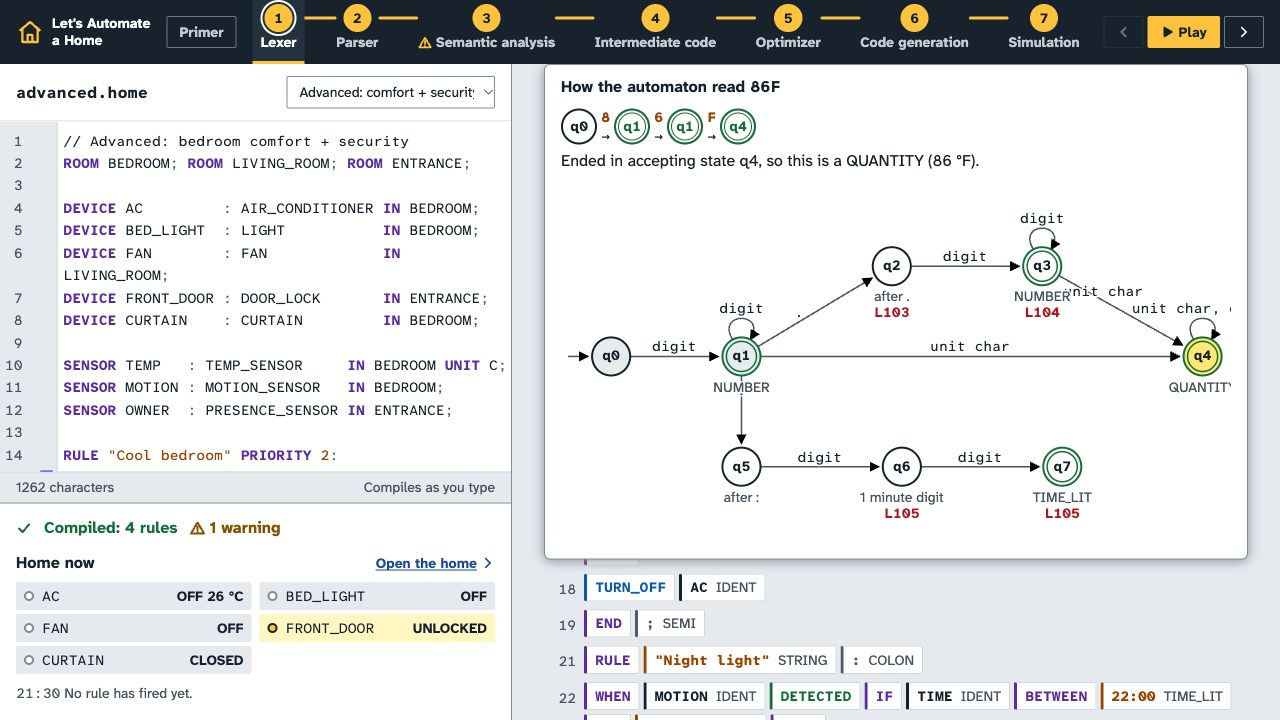
\includegraphics[width=\columnwidth]{after-lexer.jpg}
\caption{Stage 1 in the walkthrough. Selecting the token \code{86F} shows the path $q_0 \xrightarrow{8} q_1 \xrightarrow{6} q_1 \xrightarrow{F} q_4$ through the number DFA, drawn from the same data the lexer runs.}
\label{fig:lexer}
\end{figure}

The lexer recovers after an error: an unterminated string is reported and scanning resumes at the end of the line, so later tokens are still checked. Ten lexical diagnostics (L101--L110) cover illegal characters, a lone \code{!}, malformed decimals, malformed or out-of-range times, unknown units, unterminated strings and comments, and numbers above $10^9$. Carriage returns, non-breaking spaces and a leading byte-order mark are treated as whitespace.

\subsection{Phase 2: Syntax analysis}
The grammar (Listing~\ref{lst:grammar}) is stored in \code{grammar.ts}. The command \code{npm run ll1} computes FIRST and FOLLOW sets from it, builds the predictive parse table (230 entries) and reports \textbf{0 LL(1) conflicts}. Several design choices make this possible. Mandatory \code{END} on a nested \code{IF} removes the dangling-else ambiguity. Parentheses group conditions only, never arithmetic, so \code{atom} can decide on \code{"("} with one token of lookahead. The optional rule terminator is safe because \code{END} is not in FOLLOW(\code{rule}) and \code{;} is not in FIRST(\code{rule}).

\begin{lstlisting}[float=t,basicstyle=\ttfamily\tiny,caption={Core of the LL(1) grammar (EBNF).},label={lst:grammar}]
program  -> {decl} {rule} [simulate] EOF
rule     -> [RULE STRING [PRIORITY NUMBER] ":"] ruleBody [";"]
ruleBody -> IF cond [FOR duration] THEN actions [ELSE actions] [END]
          | WHEN event [IF cond] THEN actions [END]
          | AT TIME_LIT [ON days] THEN actions [END]
actions  -> action {"," action}
action   -> TURN_ON IDENT | SET IDENT IDENT TO value
          | WAIT duration | NOTIFY STRING | ...
          | IF cond THEN actions [ELSE actions] END
cond     -> andCond {OR andCond}
andCond  -> notCond {AND notCond}
notCond  -> NOT notCond | atom
atom     -> "(" cond ")" | value [atomTail]
atomTail -> relop value | IS [NOT] enumLit
          | BETWEEN value AND value
value    -> term {("+"|"-") term}
term     -> factor {("*"|"/") factor}
factor   -> NUMBER | QUANTITY | TIME_LIT | IDENT
          | "-" factor | enumLit
\end{lstlisting}

The parser is hand-written recursive descent with one function per non-terminal. It builds both a concrete parse tree (for teaching) and an abstract syntax tree whose nodes carry source spans. Operator precedence, from highest, is: unary minus; \code{* /}; \code{+ -}; relational operators, \code{IS} and \code{BETWEEN} (non-associative, so \code{20 < T < 30} is error P209); \code{NOT}; \code{AND}; \code{OR}. By default the parser stops at the first syntax error. With ``collect all errors'' enabled it uses \emph{panic-mode recovery}: it records the error, discards tokens up to a synchronizing token (\code{;}, \code{END} or the start of a rule) and resumes. Eighteen syntax diagnostics (P201--P218) give specific messages, for example P201 for a missing \code{THEN}, P208 for \code{TURN ON} written as two words, P212 for a space between a number and its unit, and P218 for nesting deep enough to threaten the call stack.

\subsection{Phase 3: Semantic analysis}\label{sec:sem}
\paragraph{Symbol table and name resolution}
A two-pass analysis first enters every room, device and sensor (or the standard-home prelude), then resolves every reference. Each entry records its kind, type, room, unit, dimension, use count and the rules that read and write it; the table is shown in the walkthrough and emitted by \code{--emit=symbols}. A catalogue of 7 device types and 6 sensor types defines the actions, states, events, attributes and value ranges each type supports.

\paragraph{Type and unit checking}
Every expression receives a type and, for quantities, a dimension. The checker rejects comparing a temperature with a power state (S308), units of different dimensions (S310), out-of-range setpoints such as \code{SET AC TEMPERATURE TO 35C} (S311, range 16--30\,\degC), actions a device does not support (S306), and actions on read-only sensors (S305). It converts \degF{} literals to \degC{} at compile time (note W410). An enum attribute resolves names against its own value set first, so in \code{SET AC MODE TO FAN}, \code{FAN} is a mode and not the device.

\paragraph{Interval analysis}
Each condition is converted to disjunctive normal form by pushing \code{NOT} inward with De~Morgan's laws and negating relational operators at the leaves. Each conjunction becomes a \emph{box}: one allowed interval set per variable, obtained by intersection. Because every atom constrains a single variable, the analysis is exact apart from comparisons between two sensors. If the condition yields no non-empty box, it can never be true (W401); if its negation yields none, it is always true (W402). Time windows that cross midnight split into two intervals. A cap on DNF size reports W416 instead of exploding exponentially.

\paragraph{Conflict detection}
Two state rules (or two rules started by the same event or time) that write opposite commands to the same device at equal priority conflict if their condition boxes intersect. The analyzer reports W404 together with a concrete \emph{witness}, a point inside the intersection, which the user can load into the simulator with one click.

\paragraph{Loop detection}
A rule-dependency graph has an edge from rule $A$ to rule $B$ when $A$ writes something $B$ reads or is triggered by. Edges are value-sensitive: \code{WHEN LIGHT TURNS ON THEN TURN\_OFF LIGHT} alone does not loop. Tarjan's algorithm finds the strongly connected components. A cycle with no guarding condition is error S317 (infinite loop); a guarded cycle is warning W407. Physical effects such as ``AC on lowers temperature'' are drawn as dashed edges and excluded from S317; otherwise the brief itself would be rejected as a self-loop. A further check catches a single rule that undoes its own state test, such as \code{IF LIGHT IS OFF THEN TURN\_ON LIGHT ELSE TURN\_OFF LIGHT}.

Overall the phase defines 25 semantic errors (S301--S325) and 16 warnings or notes (W401--W416). Several map directly to the bug classes of~\cite{brackenbury2019}: \emph{infinite loop} (S317, W407), \emph{contradictory action} such as a heater and an AC fighting around one threshold (W411), \emph{missing reversal} (W406), \emph{secure-default bias} (W412, unlocking with no presence check) and \emph{priority conflict} (W404). \emph{Repeated triggering} is prevented by design, because \code{IF} rules fire only on a false-to-true edge.

\subsection{Phase 4: Intermediate code generation}
Rules are lowered in one pass to quadruples \code{(op, arg1, arg2, result)}, numbered densely from 100 across all rules. Boolean conditions use \emph{backpatching}~\cite{dragon}: each conditional or unconditional jump is emitted with an unknown target and its index is added to a \emph{truelist} or \emph{falselist}; \code{backpatch(list, target)} fills every jump in a list once the label is known. \code{AND}, \code{OR} and \code{NOT} therefore emit no instructions of their own, only jumps, which gives short-circuit evaluation. A state rule lowers to the condition, an \code{EDGE\_TRUE} check followed by the \code{THEN} actions, and an \code{EDGE\_FALSE} check followed by the \code{ELSE} actions. Unit conversions appear explicitly, for example \code{CVT\_F\_TO\_C}. The IR is then divided into basic blocks and a control-flow graph, both of which the walkthrough displays; the backpatching itself can be replayed step by step (Fig.~\ref{fig:ir}).

\begin{figure}[t]
\centering
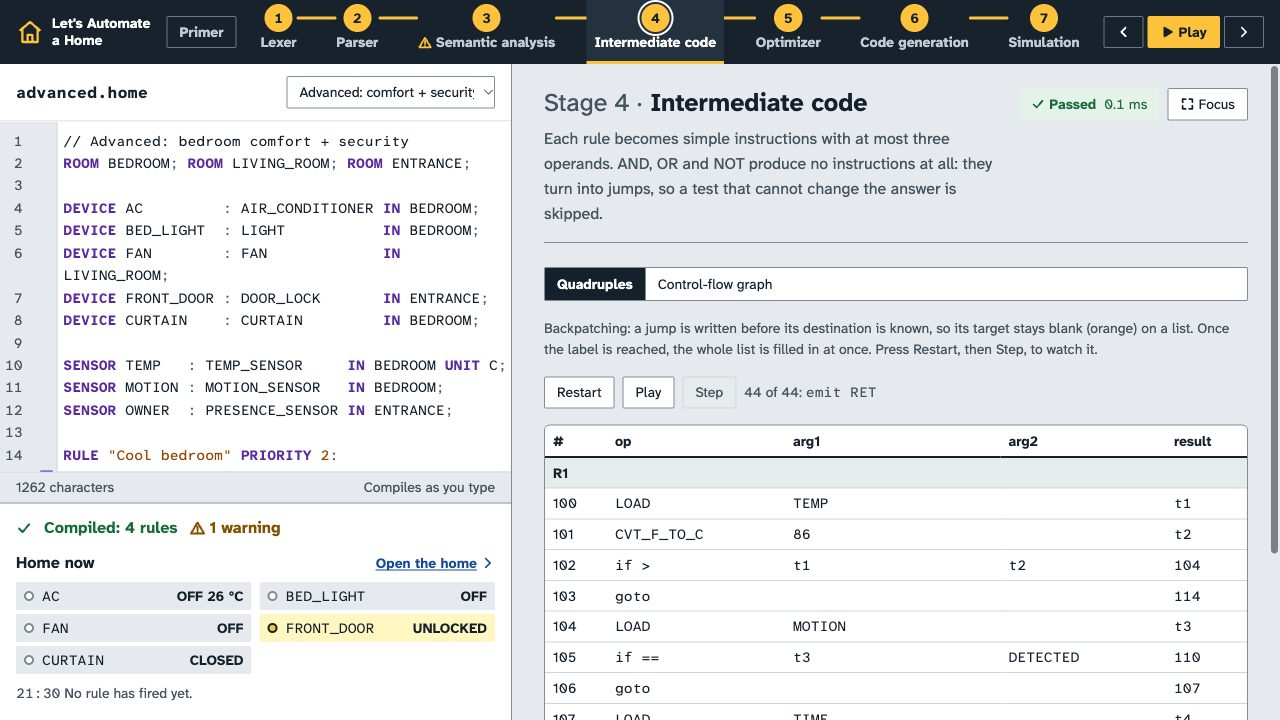
\includegraphics[width=\columnwidth]{after-ir.jpg}
\caption{Stage 4 for \code{advanced.home}: the quadruple table with step-by-step backpatching replay and a tab for the control-flow graph.}
\label{fig:ir}
\end{figure}

\subsection{Phase 5: Optimization}
Nine passes are implemented (Table~\ref{tab:opt}). Four of them rewrite conditions or whole rules, so they run on a copy of the AST, which is then re-lowered by the same IR generator; the other five run on quadruples. Each pass is a pure function and reports its changes, a before/after listing and a one-sentence safety argument that the UI displays. Two passes needed careful treatment. Common-subexpression elimination (O6) is an \emph{available-expressions} analysis with intersection at join points, because short-circuit jumps mean an earlier load may never have executed; \code{WAIT} clears the available set because values must be re-read after a delay. Redundant-action removal (O7) excludes \code{TOGGLE}, which is not idempotent.

\begin{table}[t]
\centering
\caption{Optimizer passes in run order, measured on \code{examples/optimizer.home}}
\label{tab:opt}
\footnotesize
\begin{tabular}{@{}l l l r@{}}
\toprule
Pass & Name & Level & Quads \\
\midrule
O3 & Boolean simplification & AST & 60 $\to$ 60 \\
O4 & Range merging & AST & 60 $\to$ 57 \\
O5 & Dead-rule elimination & AST & 57 $\to$ 46 \\
O9 & Rule merging & AST & 46 $\to$ 39 \\
O2 & Unit normalization & IR & 39 $\to$ 38 \\
O1 & Constant folding & IR & 38 $\to$ 37 \\
O6 & Common subexpressions & IR & 37 $\to$ 36 \\
O7 & Redundant action removal & IR & 36 $\to$ 35 \\
O8 & Jump optimization & IR & 35 $\to$ 31 \\
\midrule
\multicolumn{3}{@{}l}{Total (jumps: 16 $\to$ 4)} & 60 $\to$ 31 \\
\bottomrule
\end{tabular}
\end{table}

Examples of each: O3 rewrites \code{NOT (HUMIDITY < 40\%)} as \code{HUMIDITY >= 40\%}; O4 reduces \code{T > 26C AND T > 28C} to \code{T > 28C}; O5 removes a rule whose condition is empty by interval analysis; O9 merges neighbouring rules with the same condition while each action keeps its original rule ID for the event log; O2 turns \code{5MIN} into 300 seconds; O1 folds \code{20C + 4C} to 24 using the same rounding function as the VM; O8 replaces an \code{if ... goto L1; goto L2} pair with a single \code{ifFalse}.

\subsection{Phase 6: Code generation}
The optimized quadruples are translated into bytecode for a stack machine with 27 instructions: \code{PUSH}, \code{LOAD}, arithmetic, six comparisons, \code{IN\_WINDOW} for time windows, three jumps, \code{EDGE\_TRUE}/\code{EDGE\_FALSE}, device commands (\code{CMD}, \code{SETA}), \code{WAIT}, \code{NOTIFY} and \code{HALT}. Two opcodes, \code{STORE} and \code{LOCAL}, hold a temporary that is used more than once in a frame slot, so the savings of O6 survive into the bytecode. The output is a JSON \emph{object file} containing the rooms, the devices with their states, attributes and ranges, the sensors, a string table, a rule table (kind, priority, entry address, reads and writes) and the code. An approximate Home Assistant YAML export is also generated as a second target.

\subsection{Phase 7: Run-time simulation}
A discrete-event scheduler executes the object file. It applies the first scenario minute without events, performs an initial synchronization, and then advances to every minute, \code{WAIT} end and \code{FOR} hold end, so time rules and holds are exact. Each tick follows the cycle of Section~\ref{sec:lang}: update sensors, find triggered rules, run each in the VM, resolve commands per device by priority, commit, and treat every change as an event for the next round. Four run-time diagnostics exist: R501 (cascade deeper than 16), R502 (a non-finite value), R503 (a computed setpoint clamped to its range) and R504 (a device oscillating, defined as four power changes within five minutes). The result is an animated floor plan and a timestamped event log linked to the source lines that caused each entry.

%=====================================================================
\section{End-to-End Example}
%=====================================================================

This section traces the one-line brief \code{IF TEMPERATURE > 30 THEN TURN\_ON AC} (35 characters) through all seven phases. All listings are actual compiler output.

\paragraph{Tokens} The lexer produces 7 tokens plus \code{EOF} (Table~\ref{tab:tokens}).

\begin{table}[h]
\centering
\caption{Token stream for the brief}
\label{tab:tokens}
\footnotesize
\begin{tabular}{@{}l l l@{}}
\toprule
Type & Lexeme & Line:Col \\
\midrule
\code{IF} & \code{IF} & 1:1 \\
\code{IDENT} & \code{TEMPERATURE} & 1:4 \\
\code{GT} & \code{>} & 1:16 \\
\code{NUMBER} & \code{30} & 1:18 \\
\code{THEN} & \code{THEN} & 1:21 \\
\code{TURN\_ON} & \code{TURN\_ON} & 1:26 \\
\code{IDENT} & \code{AC} & 1:34 \\
\code{EOF} & & 1:36 \\
\bottomrule
\end{tabular}
\end{table}

\paragraph{AST} \code{Program} $\to$ \code{Rule R1 (priority 1)} with a \code{State} trigger \code{Compare(>, Ref TEMPERATURE, NumLit 30)} and one action \code{Power(TURN\_ON, Ref AC)} (Fig.~\ref{fig:parser}).

\begin{figure}[t]
\centering
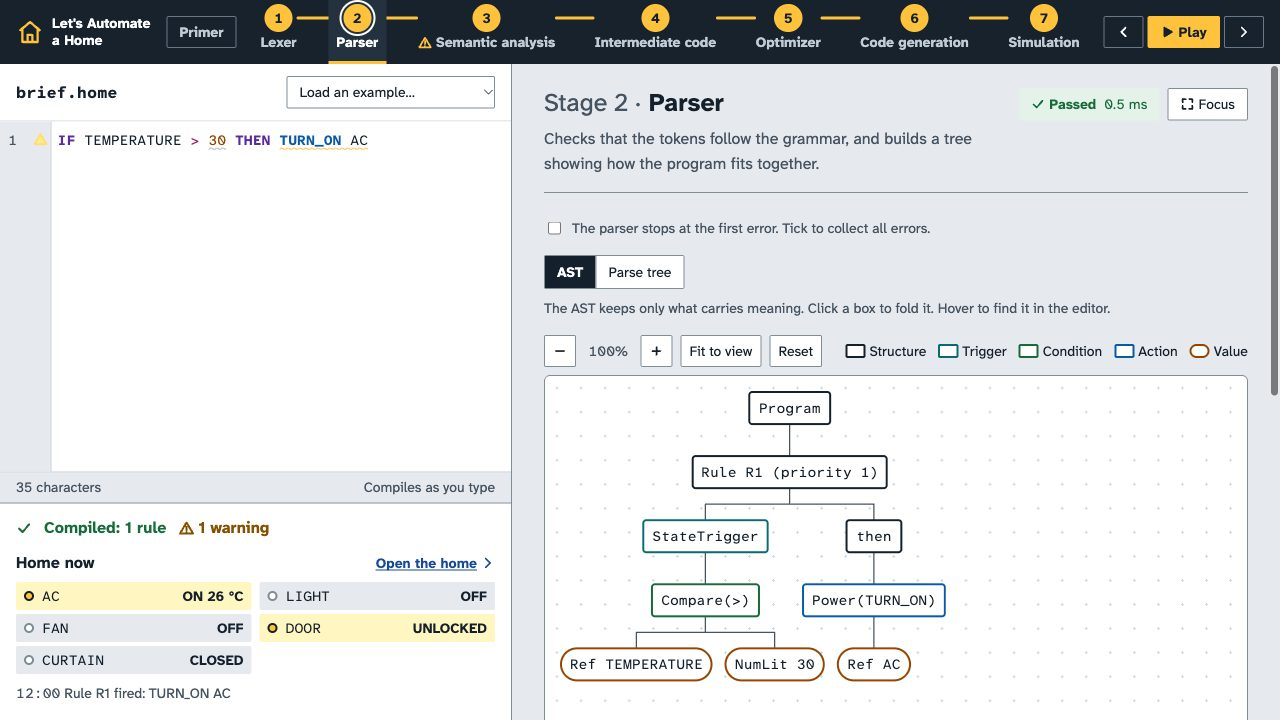
\includegraphics[width=\columnwidth]{after-parser.jpg}
\caption{Stage 2: the AST of the brief, drawn top-down. Hovering a node highlights its source span in the editor; a second tab shows the full parse tree.}
\label{fig:parser}
\end{figure}

\paragraph{Semantic analysis} \code{TEMPERATURE} resolves to a prelude sensor of type \code{TEMP\_SENSOR} (dimension temperature, unit \degC) read by R1, and \code{AC} to an \code{AIR\_CONDITIONER} written by R1. Two diagnostics are produced, neither of which stops compilation:
\begin{lstlisting}
1:18: info W415: 30 interpreted as 30 °C.
1:26: warning W406: AC is turned on by R1
      but no rule ever turns it off.
\end{lstlisting}

\paragraph{IR and backpatching} When the comparison is lowered, quad 101 is emitted with an unknown target and placed on the truelist, and quad 102 on the falselist. Reaching the \code{THEN} code performs \code{backpatch(\{101\}, 103)}; reaching the \code{ELSE} code performs \code{backpatch(\{102\}, 106)}.
\begin{lstlisting}
100 t1 := LOAD TEMPERATURE
101 if t1 > 30 goto 103
102 goto 106
103 EDGE_TRUE R1
104 CALL TURN_ON AC
105 RET
106 EDGE_FALSE R1
107 RET
\end{lstlisting}

\paragraph{Optimization} Jump optimization (O8) merges the conditional jump and the \code{goto} into one inverted jump, giving 7 quads:
\begin{lstlisting}
100 t1 := LOAD TEMPERATURE
101 ifFalse t1 > 30 goto 105
102 EDGE_TRUE R1
103 CALL TURN_ON AC
104 RET
105 EDGE_FALSE R1
106 RET
\end{lstlisting}

\paragraph{Bytecode} Nine stack-machine instructions; addresses are indexes into the code array:
\begin{lstlisting}
0 LOAD TEMPERATURE    5 CMD TURN_ON AC R1
1 PUSH 30             6 HALT
2 CMP_GT              7 EDGE_FALSE R1
3 JMP_IF_FALSE 7      8 HALT
4 EDGE_TRUE R1 0
\end{lstlisting}

\paragraph{Simulation} With no \code{SIMULATE} block the home starts live at 12:00 on Monday. Moving the temperature slider from 28\,\degC{} to 31\,\degC{} makes the condition rise from false to true, \code{EDGE\_TRUE} lets execution continue, and the log reads \code{12:00 Rule R1 fired: TURN\_ON AC}; the floor plan shows the AC switched on (Fig.~\ref{fig:overview}).

\begin{figure*}[t]
\centering
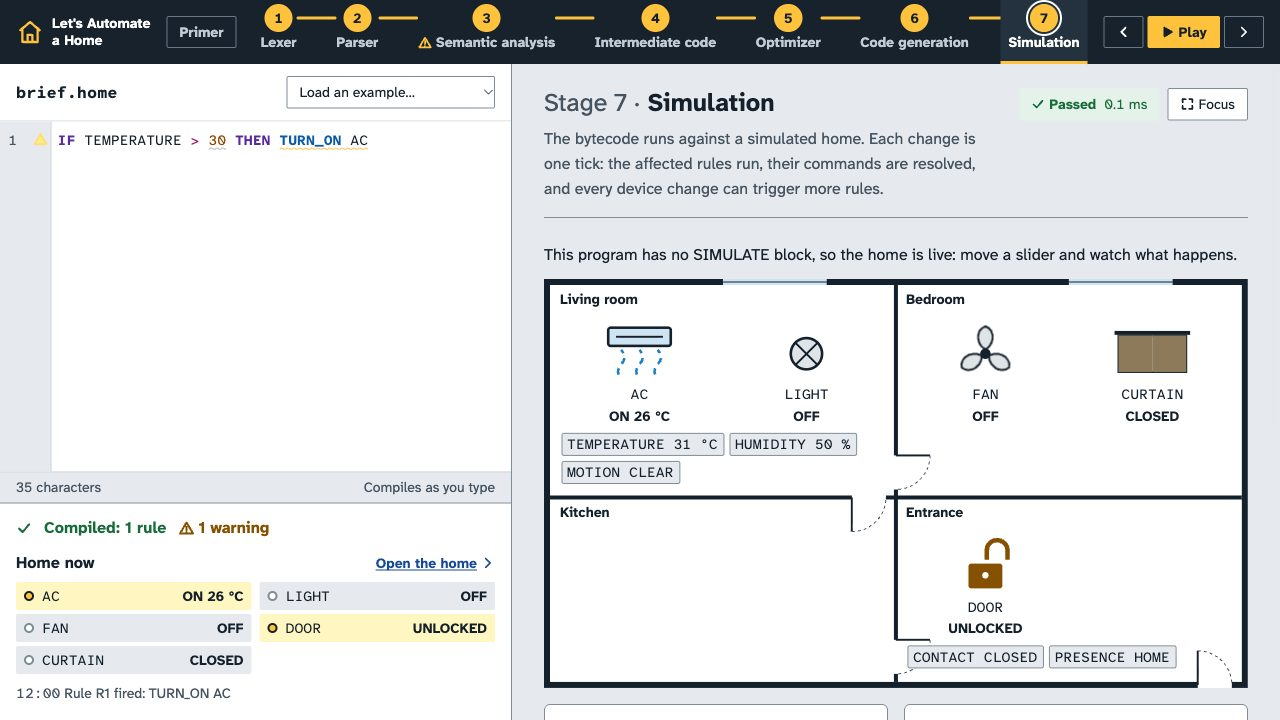
\includegraphics[width=0.78\textwidth]{after-overview.jpg}
\caption{The interactive walkthrough. The seven stages sit as stations on a wire at the top, each showing its status and time. Left: the editor and a live summary of the home. Right: Stage 7, the simulated home drawn as a floor plan, after the brief has turned on the AC.}
\label{fig:overview}
\end{figure*}

%=====================================================================
\section{Error Handling and Edge Cases}
%=====================================================================

Every diagnostic carries a code, a severity, a message, a hint and a source span. Errors stop the pipeline at their stage; warnings and notes do not. Table~\ref{tab:diag} summarizes the 74 codes. Each one is listed in the language reference with an example program. A unit test checks that the table lists every code the compiler defines, compiles every example, and checks that it produces the code of its row, so the documentation cannot drift from the compiler.

\begin{table}[t]
\centering
\caption{Diagnostic codes by phase}
\label{tab:diag}
\footnotesize
\begin{tabular}{@{}l l r >{\raggedright\arraybackslash}p{3.3cm}@{}}
\toprule
Phase & Codes & \# & Example trigger \\
\midrule
Lexical & L101--L110 & 10 & \code{AT 25:70} $\to$ L107 time out of range \\
Syntax & P201--P218 & 18 & \code{IF T > 30 TURN\_ON AC} $\to$ P201 missing \code{THEN} \\
Semantic error & S301--S325 & 25 & \code{IF TEMPERATURE > ON} $\to$ S308 type mismatch \\
Semantic warning & W401--W416 & 16 & \code{T > 30 AND T < 20} $\to$ W401 never true \\
Run time & R501--R504 & 4 & cascade deeper than 16 $\to$ R501 \\
Internal & I001 & 1 & any caught exception \\
\midrule
Total & & 74 & \\
\bottomrule
\end{tabular}
\end{table}

\begin{figure}[t]
\centering
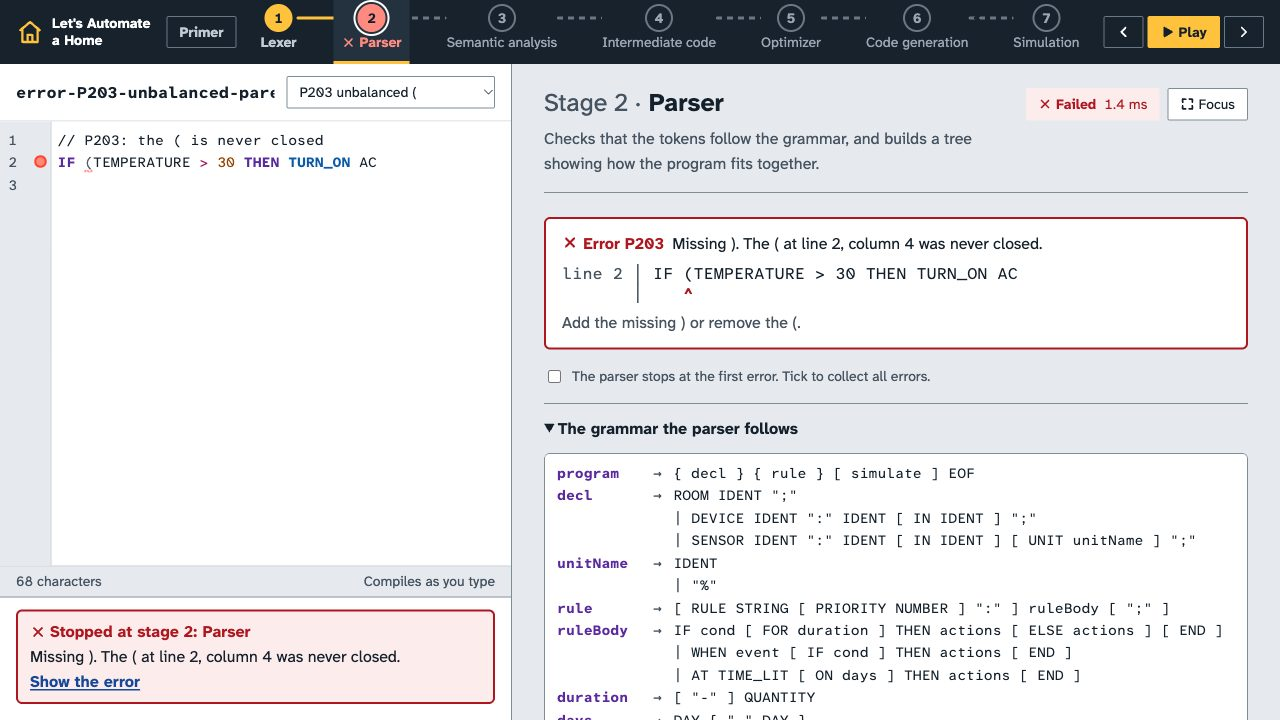
\includegraphics[width=\columnwidth]{after-failure.jpg}
\caption{A syntax error (P203, unclosed parenthesis). The wire breaks at Stage 2, later stages are greyed out, and the error box quotes the source line with a caret and a hint.}
\label{fig:failure}
\end{figure}

Representative edge cases handled include: \code{30CTHEN} (unit suffix rejected as a whole, L106); \code{PRIORITY 2:} (DFA rollback); \code{-5} (no signed literals: \code{MINUS} then \code{NUMBER}); \code{20 < T < 30} (chained comparison, P209); a nested \code{IF} without \code{END} (P213); \code{TEMP + 2F} (\degF{} arithmetic is ambiguous, S310); \code{TIME BETWEEN 22:00 AND 06:00} (wraps midnight); \code{BETWEEN 30 AND 20} on numbers (empty range, W409); literal division by zero (S324); two rules that switch each other forever (S317); and 500 nested parentheses (P218 instead of a stack overflow). Fig.~\ref{fig:failure} shows how an error appears in the interface.

%=====================================================================
\section{Interactive Visualization}\label{sec:ui}
%=====================================================================

The web application compiles on every keystroke and exposes each phase as a numbered stage, opened from a rail at the top (Fig.~\ref{fig:overview}). The rail is lit as far as the program got and broken at a failure. A Play button steps through the stages with their animations, and Focus enlarges one stage for a projector. Text uses the Atkinson Hyperlegible typefaces so that similar characters stay distinct from the back of a room.

\begin{itemize}
  \item \textbf{Lexer:} token stream with categories, and the DFA diagram with the exact path taken for any selected token (Fig.~\ref{fig:lexer}).
  \item \textbf{Parser:} AST and parse tree with fold, zoom and pan, linked both ways to the editor; the grammar; FIRST/FOLLOW sets and the parse table; a grammar stepper (Fig.~\ref{fig:parser}).
  \item \textbf{Semantic analysis:} symbol table, diagnostics, number lines showing the true set of each condition, a conflict matrix with loadable witnesses, and the rule-dependency graph with its strongly connected components.
  \item \textbf{Intermediate code:} quadruple table with a step-by-step backpatching replay, and the control-flow graph (Fig.~\ref{fig:ir}).
  \item \textbf{Optimizer:} per-pass diffs with the safety reason for each change, and totals.
  \item \textbf{Code generation:} bytecode listing, a step-through debugger that shows the VM stack, the JSON object file and the Home Assistant export.
  \item \textbf{Simulation:} the floor plan, sensor controls grouped by room, a time scrubber, scenario playback at 1$\times$, 10$\times$ and 60$\times$, and the event log linked to the editor (Fig.~\ref{fig:overview}).
\end{itemize}

When a half-typed program fails, the last working home remains on screen, dimmed, and a new failure is shown only after a 500\,ms pause so the page does not flicker while the user is typing. Twenty-one preset programs can be loaded from a menu: eight valid programs and thirteen that each demonstrate one error or warning.

%=====================================================================
\section{Testing and Verification}\label{sec:testing}
%=====================================================================

\begin{table*}[t]
\centering
\caption{Module ownership (matches the repository's commit history)}
\label{tab:contrib}
\footnotesize
\begin{tabular}{@{}l l >{\raggedright\arraybackslash}p{10.6cm}@{}}
\toprule
Member & Phase owned & Main files \\
\midrule
Deepanshu Mehta & Lexer, scaffold, UI shell & \code{src/compiler/lexer/}, stage interfaces, \code{src/ui/App.tsx}, \code{Editor.tsx}, \code{styles/}, \code{viz/DfaDiagram.tsx}, \code{viz/FloorPlan.tsx}, \code{tests/e2e/}, CI \\
Vishesh Rao & Parser & \code{src/compiler/parser/}, \code{scripts/ll1.ts}, \code{src/ui/trees.ts}, \code{viz/TreeView.tsx}, \code{cards/ParserCard.tsx} \\
Manu Vahan & Semantic analysis & \code{src/compiler/semantic/}, \code{cards/SemanticCard.tsx}, \code{viz/GraphView.tsx}, \code{viz/NumberLine.tsx} \\
Pranay Vishwakarma & IR and optimizer & \code{src/compiler/ir/}, \code{src/compiler/opt/}, \code{cards/IrCard.tsx}, \code{cards/OptimizerCard.tsx}, \code{DiffView} \\
Ankush Yadav & Codegen, VM, simulator & \code{src/compiler/codegen/}, \code{src/compiler/runtime/}, \code{src/compiler/index.ts}, \code{src/cli/}, golden and differential tests, \code{CodegenCard}, \code{SimulationCard} \\
\bottomrule
\end{tabular}
\end{table*}

\subsection{Test suites}
\begin{itemize}
  \item \textbf{Unit tests} for every phase: lexer, LL(1) proof, parser, semantic checks, interval and loop analysis, IR, optimizer, VM, simulator, Home Assistant export, boundaries and design tokens.
  \item \textbf{Golden tests:} each of the 21 example programs is compiled and its tokens, AST, symbols, IR, optimized IR, bytecode and simulation log are compared with stored snapshots.
  \item \textbf{Error table:} programs that must each produce one specific diagnostic, plus the test that compiles every example in the diagnostics table of the language reference.
  \item \textbf{Fuzz tests:} random token streams, random characters, mutated examples (a token deleted, duplicated or swapped), pathological nesting and a 200-term condition. The compiler must never throw, never report I001, and every span must be valid.
  \item \textbf{Browser tests} (Playwright): all 21 presets load and render every stage, keyboard navigation works, and fast typing does not freeze the editor.
\end{itemize}
In total, 1104 unit, golden and property tests in 17 files pass in about 3\,s, and 56 browser tests pass.

\subsection{Differential testing of the optimizer}
The strongest evidence that the optimizations are safe is a three-way differential test. Each program is executed by (a) an independent AST interpreter that uses no IR, optimizer or VM; (b) the VM running unoptimized bytecode; and (c) the VM running optimized bytecode. All three must produce identical event logs and identical final states. The test runs on every example, on 39 programs written to stress individual passes and timing rules, and on 400 randomly generated programs.

To test the test, 13 parts of the compiler were deliberately broken. Initially only 6 of the 13 sabotages were caught, because the test programs never hit a threshold exactly and the oracle shared its time-window code with the VM. After both weaknesses were fixed, all 13 sabotages make the suite fail. The exercise also exposed a genuine logging difference in R503, which was then fixed.

\subsection{Performance}
Table~\ref{tab:perf} gives the mean time for a complete seven-stage compilation, averaged over 200 runs after warm-up on an Apple M2 laptop under Node.js~22. Compilation is fast enough to run on every keystroke.

\begin{table}[t]
\centering
\caption{End-to-end compile time (all seven stages)}
\label{tab:perf}
\footnotesize
\begin{tabular}{@{}l r r r@{}}
\toprule
Program & Chars & Tokens & Time (ms) \\
\midrule
\code{brief} & 35 & 7 & 0.32 \\
\code{living-room} & 749 & 147 & 1.12 \\
\code{night-security} & 1088 & 175 & 2.95 \\
\code{optimizer} & 1531 & 150 & 1.21 \\
\code{advanced} & 1262 & 223 & 3.72 \\
\bottomrule
\end{tabular}
\end{table}

%=====================================================================
\section{Individual Member Contributions}
%=====================================================================

Each member built and owns one stage of the compiler together with its user-interface card and its tests. Table~\ref{tab:contrib} lists the files each member wrote; it matches the commit history of the repository.


\textbf{Deepanshu Mehta} set up the project and the shared stage interfaces that let the five phases be built in parallel; implemented the lexer (the six data-driven DFAs, the maximal-munch runner, keyword and unit tables, lexical diagnostics and their tests); wrote the language reference; and built the application shell: the editor, design tokens and styles, the DFA diagram, the floor-plan view, the error table with the diagnostics and boundary tests, the browser tests and the CI workflow. Deepanshu also led the end-to-end review that fixed defects across stages.

\textbf{Vishesh Rao} wrote the grammar as data, the FIRST/FOLLOW computation and LL(1) proof, the recursive-descent parser with panic-mode recovery, the AST and parse-tree builders, the parser error examples, and the Parser stage with its tree views.

\textbf{Manu Vahan} implemented the semantic analyzer: the two-pass symbol table, the type and unit checker, interval analysis, conflict detection, the rule-dependency graph with S317 loop detection, the semantic tests, and the Semantic stage with its graph and number-line views.

\textbf{Pranay Vishwakarma} implemented quadruple generation with backpatching, basic blocks and the control-flow graph, the optimizer pipeline and all nine passes, their tests, and the Intermediate code and Optimizer stages with the per-pass diff view.

\textbf{Ankush Yadav} implemented the bytecode emitter, the object-file format, the stack VM and debugger, the scheduler and simulator, the AST interpreter used as the test oracle, the Home Assistant export, the pipeline entry point and command-line tool, the golden and differential tests, and the Code generation and Simulation stages.

%=====================================================================
\section{Limitations and Future Scope}
%=====================================================================

\paragraph{Limitations} The interval analysis is exact only for single-variable atoms; comparisons between two sensors are treated as unknown. Physical effects (an AC lowering the temperature) are modelled as dashed dependency edges for warnings, not simulated physically. The Home Assistant export is approximate, because some HomeLang semantics such as edge-triggered \code{ELSE} have no direct YAML equivalent. Parentheses cannot group arithmetic, a deliberate restriction that keeps the grammar LL(1).

\paragraph{Future scope}
\begin{itemize}
  \item \textbf{Multi-target code generation:} exact back ends for Home Assistant, openHAB rules and SmartThings, and a native target for microcontrollers such as the ESP32 that run the bytecode directly.
  \item \textbf{Stronger analysis:} relational domains (octagons or polyhedra) for comparisons between sensors, and export of rules to a model checker for temporal properties in the style of IotSan and AutoTap~\cite{iotsan,autotap}.
  \item \textbf{More optimization:} a peephole pass over the bytecode, a register-based instruction set, and merging of rules that are not neighbours when no priority tie or notification order can change.
  \item \textbf{Language features:} user-defined scenes, functions, arrays of devices (\code{ALL LIGHTS IN BEDROOM}), and sunrise/sunset times.
  \item \textbf{Live devices:} connecting the runtime to real devices through MQTT or Matter instead of the simulator.
  \item \textbf{Teaching aids:} an LR(1) parsing view for comparison with LL(1), and a guided mode that asks the student to predict the next quad or token.
\end{itemize}

%=====================================================================
\section{Conclusion}
%=====================================================================

HomeLang shows that a small, well-specified domain language can exercise the full compiler pipeline in depth. Each phase follows the classical theory directly: DFAs with maximal munch, an LL(1) grammar proven free of conflicts, a typed and dimension-aware symbol table, interval analysis, backpatched quadruples, provably safe optimizations, and a stack machine. Because the automata and grammar are data and every phase is a pure function, the same objects drive both the compiler and its visualization, and every intermediate state can be shown, tested and explained. The three-way differential test, validated by deliberate sabotage, gives strong evidence that the generated code is correct.

\section*{Repository and Setup}
Source:\\ \url{https://github.com/Deepanshu-Mehta/HomeLang-CompilerDesign}\\ Requirements: Node.js 22 and npm. Commands: \code{npm install}; \code{npm run dev} (walkthrough); \code{npm test}; \code{npm run test:e2e} (needs Google Chrome); \code{npm run build}; \code{npm run ll1}.

\begin{thebibliography}{00}
\bibitem{ur2014} B.~Ur, E.~McManus, M.~Pak~Yong~Ho, and M.~L.~Littman, ``Practical trigger-action programming in the smart home,'' in \textit{Proc. ACM CHI Conf. Human Factors in Computing Systems}, 2014, pp.~803--812.
\bibitem{brackenbury2019} W.~Brackenbury, A.~Deora, J.~Ritchey, J.~Vallee, W.~He, G.~Wang, M.~L.~Littman, and B.~Ur, ``How users interpret bugs in trigger-action programming,'' in \textit{Proc. ACM CHI Conf. Human Factors in Computing Systems}, 2019.
\bibitem{iotsan} D.~T.~Nguyen, C.~Song, Z.~Qian, S.~V.~Krishnamurthy, E.~J.~M.~Colbert, and P.~McDaniel, ``IotSan: Fortifying the safety of IoT systems,'' in \textit{Proc. 14th Int. Conf. Emerging Networking EXperiments and Technologies (CoNEXT)}, 2018, pp.~191--203.
\bibitem{autotap} L.~Zhang, W.~He, J.~Martinez, N.~Brackenbury, S.~Lu, and B.~Ur, ``AutoTap: Synthesizing and repairing trigger-action programs using LTL properties,'' in \textit{Proc. 41st Int. Conf. Software Engineering (ICSE)}, 2019, pp.~281--291.
\bibitem{dragon} A.~V.~Aho, M.~S.~Lam, R.~Sethi, and J.~D.~Ullman, \textit{Compilers: Principles, Techniques, and Tools}, 2nd~ed. Boston, MA, USA: Addison-Wesley, 2006.
\bibitem{nystrom} R.~Nystrom, \textit{Crafting Interpreters}. Genever Benning, 2021.
\bibitem{tarjan} R.~E.~Tarjan, ``Depth-first search and linear graph algorithms,'' \textit{SIAM J. Comput.}, vol.~1, no.~2, pp.~146--160, 1972.
\bibitem{homeassistant} Home Assistant, ``Automation triggers,'' documentation. [Online]. Available: \url{https://www.home-assistant.io/docs/automation/trigger/}
\bibitem{matter} Connectivity Standards Alliance, \textit{Matter Application Cluster Specification}. [Online]. Available: \url{https://csa-iot.org/developer-resource/specifications-download-request/}
\end{thebibliography}

\end{document}
